%%p01
Calcula el valor de ``$x$''.
\begin{figure}[h]
	\begin{tikzpicture}[thick]
		\def\r{2.5}
		\tkzDefPoint(-22:\r){v1}
		\tkzDefPoint(-158:\r){v2}
		\tkzDefPoint(66:\r){v3}
		\tkzFillAngles[size=6mm,fill=yellow,opacity=.2](v1,v2,v3 v2,v3,v1)
		\tkzMarkAngles[size=6mm,mark=none](v1,v2,v3 v2,v3,v1)
		\tkzLabelAngle(v1,v2,v3){$x$}
		\tkzLabelAngle(v2,v3,v1){$68\dg$}
		\tkzDrawPolygon(v1,v2,v3)
		\tkzMarkSegments[mark=||](v1,v2 v2,v3)
	\end{tikzpicture}
\end{figure}
%%r01
$44\dg$
%%p02.sp
\begin{mini}
	Calcula la suma de las medidas de los \'angulos interiores de:
	\begin{center}
		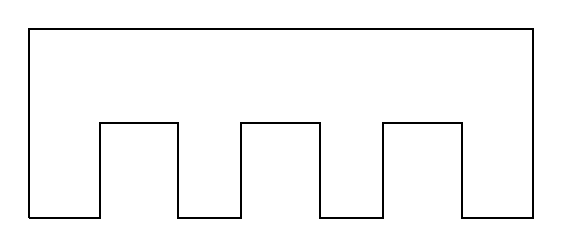
\begin{tikzpicture}[thick]
			\def\x{.8}
			\def\y{.9}
			\def\z{1}
			\def\w{1.2}
			\draw (0,0) -| (\y,\w) -| ++ (\z,-\w) -| ++ (\x,\w) -| ++ (\z,-\w) -| ++ (\x,\w) -| ++ (\z,-\w) -| ++ (\y,2*\w) -| (0,0);
		\end{tikzpicture}
	\end{center}
\end{mini}
%%a02
\begin{task}
	* $2520\dg$
	* $1440\dg$
	* $900\dg$
	* $2880\dg$
\end{task}
%%r02
$2520\dg$
%%p03.sp
\begin{mini}
	En un tri\'angulo is\'osceles, la suma de dos \'angulos distintos es igual a $110\dg$. Entonces la suma de los \'angulos de la base es:
\end{mini}
%%a03
\begin{task}
	* $150\dg$
	* $146\dg$
	* $140\dg$
	* $136\dg$
\end{task}
%%r03
$140\dg$
%%p04.sp
\begin{mini}[.75]
	En un $\triangle ABC$, $AB=BC$ y $\text{m}\dang B=108\dg$. Calcular la medida del \'angulo exterior en el v\'ertice ``$C$''.
	\begin{center}
		\begin{tikzpicture}[thick]
			\def\r{3.6}
			\tkzDefPoint(162:\r){A}
			\tkzDefPoint(0,\r){B}
			\tkzDefPoint(18:\r){C}
			\tkzDefPointOnLine[pos=1.2](A,C)
			\tkzGetPoint{D}
			\tkzFillAngles[size=5mm,fill=yellow,opacity=.2](A,B,C B,C,A C,A,B)
			\tkzFillAngle[size=3mm,fill=yellow,opacity=.2](D,C,B)
			\tkzMarkAngles[size=5mm,mark=none](A,B,C B,C,A C,A,B)
			\tkzMarkAngle[size=3mm,mark=none](D,C,B)
			\tkzLabelAngles[pos=.8](B,C,A C,A,B){$\alpha$}
			\tkzLabelAngle[pos=.8](A,B,C){$108\dg$}
			\tkzLabelAngle[pos=.55](D,C,B){$x$}
			\tkzDrawPolySeg(D,A,B,C)
			\tkzDefMidPoint(A,B)
			\tkzGetPoint{M}
			\tkzDefMidPoint(B,C)
			\tkzGetPoint{N}
			\tkzDrawPoints[size=6.5,color=yellow!50!orange](M,N)
			\tkzLabelPoints[below left](A)
			\tkzLabelPoints[above](B)
			\tkzLabelPoints[below](C)
		\end{tikzpicture}
	\end{center}
\end{mini}
%%a04
\begin{task}
	* $89\dg$
	* $124\dg$
	* $136\dg$
	* $144\dg$
\end{task}
%%r04
$144\dg$
%%p05.sp
\begin{tabular}{c}
	Si la figura es un pol\'igono regular, hallar ``$x$''. \vspace{5pt} \\
	\begin{tikzpicture}[thick]
		\tkzDefPoint(0,0){P0}
		\tkzDefPoint(112.5:2){P1}
		\tkzDefRegPolygon[sides=8](P0,P1)
		\tkzFillAngle[size=3mm,fill=yellow,opacity=.2](P3,P2,P1)
		\tkzMarkAngle[size=3mm,mark=none](P3,P2,P1)
		\tkzLabelAngle[pos=.6](P3,P2,P1){$x$}
		\tkzDrawPolygon(P1,P...,P8)
	\end{tikzpicture}
\end{tabular}
%%a05
\begin{task}
	* $120\dg$
	* $145\dg$
	* $140\dg$
	* $135\dg$
\end{task}
%%r05
$135\dg$
%%p06
Calcula el valor de ``$\alpha$''.
\begin{figure}[h]
	\begin{tikzpicture}[thick]
		\def\r{3}
		\tkzDefPoint(-165:\r){A}
		\tkzDefPoint(59:\r){B}
		\tkzDefPoint(-15:\r){C}
		\tkzDefPointOnLine[pos=1.2](A,C)
		\tkzGetPoint{D}
		\tkzFillAngles[size=5mm,fill=yellow,opacity=.2](C,A,B A,B,C D,C,B)
		\tkzMarkAngles[size=5mm,mark=none](C,A,B A,B,C D,C,B)
		\tkzLabelAngles[pos=1](C,A,B){$37\dg$}
		\tkzLabelAngle[pos=.9](A,B,C){$\alpha$}
		\tkzLabelAngle[pos=1](D,C,B){$112\dg$}
		\tkzDrawPolySeg(D,A,B,C)
	\end{tikzpicture}
\end{figure}
%%a06
\begin{task}
	* $78\dg$
	* $75\dg$
	* $73\dg$
	* $74\dg$
\end{task}
%%r06
$75\dg$
%%p07.sp
\begin{mini}
	Calcula el n\'umero total de diagonales que se pueden trazar en la siguiente figura:
	\begin{center}
		\begin{tikzpicture}[thick]
			\def\x{1.4}
			\def\y{1.5}
			\tkzDefPoints{-\x/0/A,\x/0/B}
			\tkzDefSquare(A,B)
			\tkzGetPoints{C}{D}
			\tkzDefPoints{-\x/\y/E,\x/\y/F}
			\tkzDefEquilateral(A,E)
			\tkzGetPoint{G}
			\tkzDefEquilateral(F,B)
			\tkzGetPoint{H}
			\tkzDrawPolygon(A,B,F,H,C,D,G,E)
		\end{tikzpicture}
	\end{center}
\end{mini}
%%a07
\begin{task}
	* $21$
	* $23$
	* $28$
	* $20$
\end{task}
%%r07
$20$
%%p08
Calcula el valor de ``$x$''.
\begin{figure}[h]
	\begin{tikzpicture}[thick]
		\def\r{3}
		\def\a{-3}
		\tkzDefPoint(\a+146:\r){A1}
		\tkzDefPoint(\a+184:\r){B}
		\tkzDefPointOnLine[pos=1.6](B,A1)
		\tkzGetPoint{A}
		\tkzDefPoint(\a-110:\r){C}
		\tkzDefPoint(\a:\r){D1}
		\tkzDefPoint(\a+30:\r){E1}
		\tkzDefParallelogram(A,A1,E1)
		\tkzGetPoint{P1}
		\tkzInterLL(A,P1)(D1,E1)
		\tkzGetPoint{E2}
		\tkzDefPointOnLine[pos=.9](A,E2)
		\tkzGetPoint{E}
		\tkzDefParallelogram(D1,E2,E)
		\tkzGetPoint{P2}
		\tkzInterLL(E,P2)(C,D1)
		\tkzGetPoint{D}
		\tkzFillAngles[size=5mm,fill=yellow,opacity=.2](B,A,E A,E,D E,D,C D,C,B C,B,A)
		\tkzMarkAngles[size=5mm,mark=none](B,A,E A,E,D E,D,C D,C,B C,B,A)
		\tkzLabelAngles[pos=1.1](B,A,E){$13x-53\dg$}
		\tkzLabelAngle[pos=1.4](C,B,A){$14x-40\dg$}
		\tkzLabelAngle[pos=1](D,C,B){$6x+20\dg$}
		\tkzLabelAngle[pos=1.3](E,D,C){$14x-58\dg$}
		\tkzLabelAngle[pos=1.1](A,E,D){$5x+47\dg$}
		\tkzDrawPolygon(A,B,C,D,E)
		\tkzLabelPoints[above left](A)
		\tkzLabelPoints[left](B)
		\tkzLabelPoints[below](C)
		\tkzLabelPoints[right](D)
		\tkzLabelPoints[above right](E)
	\end{tikzpicture}
\end{figure}
%%a08
\begin{enum}
	* $14\dg$
	* $13\dg$
	* $12\dg$
	* $15\dg$
\end{enum}
%%r08
$12\dg$
%%p09
\begin{tabular}{c}
	Si el tri\'angulo $ABC$ es equil\'atero, calcular $\text{m}\dang BDC$. \vspace{5pt} \\
	\begin{tikzpicture}[thick]
		\def\r{5}
		\tkzDefPoint(-120:\r){A}
		\tkzDefPoint(0,0){B}
		\tkzDefPoint(-60:\r){C}
		\tkzDefPoint(-100:1){P}
		\tkzInterLL(B,P)(A,C)
		\tkzGetPoint{D}
		\tkzFillAngle[size=8mm,fill=yellow,opacity=.2](A,B,D)
		\tkzMarkAngle[size=8mm,mark=none](A,B,D)
		\tkzLabelAngle[pos=1.7](A,B,D){$20\dg$}
		\tkzDrawPolygon(A,B,C)
		\tkzDrawSegment(B,D)
		\tkzLabelPoints[below left](A)
		\tkzLabelPoints[above](B)
		\tkzLabelPoints[below right](C)
		\tkzLabelPoints[below](D)
	\end{tikzpicture}
\end{tabular}
%%a09
\begin{task}
	* $70\dg$
	* $80\dg$
	* $90\dg$
	* $75\dg$
\end{task}
%%r09
$80\dg$
%%p10
Calcula el valor de ``$x$'' en el gr\'afico mostrado.
%%a10
\begin{task}
	* $30\dg$
	* $45\dg$
	* $54\dg$
	* $36\dg$
\end{task}
%%r10
$45\dg$
%%p11.sp
\begin{mini}
	El per\'imetro del tri\'angulo es de $\ce{20cm}$. ¿Cu\'anto mide el lado $AC$?
	\begin{center}
		\begin{tikzpicture}[thick]
			\def\r{3}
			\def\a{16.6}
			\tkzDefPoint(\a+146.8:\r){A}
			\tkzDefPoint(\a:\r){B}
			\tkzDefPoint(\a+50.42:\r){C}
			\draw (A) node[below left] {$A$} -- node[below] {$x+5$} (B) node[below right] {$B$} -- node[above right] {$x$} (C) node[above] {$C$} -- node[above left] {$x+3$} (A);
		\end{tikzpicture}
	\end{center}
\end{mini}
%%a11
\begin{task}
	* $\ce{5cm}$
	* $\ce{2cm}$
	* $\ce{7cm}$
	* $\ce{6cm}$
\end{task}
%%r11
$\ce{7cm}$
%%p12
Calcula el valor de ``$x$''.
%%a12
\begin{task}
	* $10\dg$
	* $4\dg$
	* $25\dg$
	* $7\dg$
\end{task}
%%r12
$25\dg$
%%p13
En la figura, $AB=BC=CD$. Calcular el valor de ``$\alpha$''.
%%a13
\begin{task}
	* $32\dg$
	* $68\dg$
	* $44\dg$
	* $72\dg$
\end{task}
%%r13
$68\dg$
%%p14.sp
\begin{mini}
	Hallar la suma de los n\'umeros de diagonales de un non\'agono y de un endec\'agono.
\end{mini}
%%a14
\begin{task}
	* $27$
	* $44$
	* $71$
	* $69$
\end{task}
%%r14
$71$
%%p15
Caucular ``$x$'' en:
%%a15
\begin{task}
	* $92\dg$
	* $80\dg$
	* $88\dg$
	* $100\dg$
\end{task}
%%r15
$88\dg$
